\documentclass[twoside]{book}

% Packages required by doxygen
\usepackage{calc}
\usepackage{doxygen}
\usepackage{graphicx}
\usepackage[utf8]{inputenc}
\usepackage{makeidx}
\usepackage{multicol}
\usepackage{multirow}
\usepackage{textcomp}
\usepackage[table]{xcolor}

% NLS support packages
\usepackage[T2A]{fontenc}
\usepackage[czech]{babel}

% Font selection
\usepackage[T1]{fontenc}
\usepackage{mathptmx}
\usepackage[scaled=.90]{helvet}
\usepackage{courier}
\usepackage{amssymb}
\usepackage{sectsty}
\renewcommand{\familydefault}{\sfdefault}
\allsectionsfont{%
  \fontseries{bc}\selectfont%
  \color{darkgray}%
}
\renewcommand{\DoxyLabelFont}{%
  \fontseries{bc}\selectfont%
  \color{darkgray}%
}

% Page & text layout
\usepackage{geometry}
\geometry{%
  a4paper,%
  top=2.5cm,%
  bottom=2.5cm,%
  left=2.5cm,%
  right=2.5cm%
}
\tolerance=750
\hfuzz=15pt
\hbadness=750
\setlength{\emergencystretch}{15pt}
\setlength{\parindent}{0cm}
\setlength{\parskip}{0.2cm}
\makeatletter
\renewcommand{\paragraph}{%
  \@startsection{paragraph}{4}{0ex}{-1.0ex}{1.0ex}{%
    \normalfont\normalsize\bfseries\SS@parafont%
  }%
}
\renewcommand{\subparagraph}{%
  \@startsection{subparagraph}{5}{0ex}{-1.0ex}{1.0ex}{%
    \normalfont\normalsize\bfseries\SS@subparafont%
  }%
}
\makeatother

% Headers & footers
\usepackage{fancyhdr}
\pagestyle{fancyplain}
\fancyhead[LE]{\fancyplain{}{\bfseries\thepage}}
\fancyhead[CE]{\fancyplain{}{}}
\fancyhead[RE]{\fancyplain{}{\bfseries\leftmark}}
\fancyhead[LO]{\fancyplain{}{\bfseries\rightmark}}
\fancyhead[CO]{\fancyplain{}{}}
\fancyhead[RO]{\fancyplain{}{\bfseries\thepage}}
\fancyfoot[LE]{\fancyplain{}{}}
\fancyfoot[CE]{\fancyplain{}{}}
\fancyfoot[RE]{\fancyplain{}{\bfseries\scriptsize Generováno ne 21. zář 2014 12.\-20\-:59 pro projekt Med\-Dbase for media programem Doxygen }}
\fancyfoot[LO]{\fancyplain{}{\bfseries\scriptsize Generováno ne 21. zář 2014 12.\-20\-:59 pro projekt Med\-Dbase for media programem Doxygen }}
\fancyfoot[CO]{\fancyplain{}{}}
\fancyfoot[RO]{\fancyplain{}{}}
\renewcommand{\footrulewidth}{0.4pt}
\renewcommand{\chaptermark}[1]{%
  \markboth{#1}{}%
}
\renewcommand{\sectionmark}[1]{%
  \markright{\thesection\ #1}%
}

% Indices & bibliography
\usepackage{natbib}
\usepackage[titles]{tocloft}
\setcounter{tocdepth}{3}
\setcounter{secnumdepth}{5}
\makeindex

% Hyperlinks (required, but should be loaded last)
\usepackage{ifpdf}
\ifpdf
  \usepackage[pdftex,pagebackref=true]{hyperref}
\else
  \usepackage[ps2pdf,pagebackref=true]{hyperref}
\fi
\hypersetup{%
  colorlinks=true,%
  linkcolor=blue,%
  citecolor=blue,%
  unicode%
}

% Custom commands
\newcommand{\clearemptydoublepage}{%
  \newpage{\pagestyle{empty}\cleardoublepage}%
}


%===== C O N T E N T S =====

\begin{document}

% Titlepage & ToC
\hypersetup{pageanchor=false}
\pagenumbering{roman}
\begin{titlepage}
\vspace*{7cm}
\begin{center}%
{\Large Med\-Dbase for media }\\
\vspace*{1cm}
{\large Generováno programem Doxygen 1.8.6}\\
\vspace*{0.5cm}
{\small ne 21. zář 2014 12.20:59}\\
\end{center}
\end{titlepage}
\clearemptydoublepage
\tableofcontents
\clearemptydoublepage
\pagenumbering{arabic}
\hypersetup{pageanchor=true}

%--- Begin generated contents ---
\chapter{Documentation}
\label{index}\hypertarget{index}{}\hypertarget{index_About}{}\section{About}\label{index_About}
Use make to install.

Small app for indexing C\-Ds, U\-S\-B Flashes, ...\hypertarget{index_Contact}{}\section{Contact}\label{index_Contact}
Development guided by Martin Beránek \href{mailto:martin.beranek112@gmail.com}{\tt martin.\-beranek112@gmail.\-com} 
\chapter{medi\-Dbase}
\label{d0/d30/md_README}
\hypertarget{d0/d30/md_README}{}
Small app to index and prepare documentation about cdroms, ... 
\chapter{Rejstřík hierarchie tříd}
\section{Hierarchie tříd}
Zde naleznete seznam, vyjadřující vztah dědičnosti tříd. Je seřazen přibližně (ale ne úplně) podle abecedy\-:\begin{DoxyCompactList}
\item \contentsline{section}{main.\-Chdir}{\pageref{d2/dbd/classmain_1_1Chdir}}{}
\item \contentsline{section}{D\-B\-Hand.\-D\-B\-Hand}{\pageref{df/d86/classDBHand_1_1DBHand}}{}
\item \contentsline{section}{Indx.\-Indx}{\pageref{d4/d70/classIndx_1_1Indx}}{}
\item object\begin{DoxyCompactList}
\item \contentsline{section}{mn\-Window.\-App}{\pageref{d4/d8e/classmnWindow_1_1App}}{}
\begin{DoxyCompactList}
\item \contentsline{section}{mn\-Window.\-mn\-Item}{\pageref{db/dee/classmnWindow_1_1mnItem}}{}
\end{DoxyCompactList}
\end{DoxyCompactList}
\item \contentsline{section}{Sys\-Mnt.\-Sys\-Mnt}{\pageref{de/d04/classSysMnt_1_1SysMnt}}{}
\end{DoxyCompactList}

\chapter{Rejstřík tříd}
\section{Seznam tříd}
Následující seznam obsahuje především identifikace tříd, ale nacházejí se zde i další netriviální prvky, jako jsou struktury (struct), unie (union) a rozhraní (interface). V seznamu jsou uvedeny jejich stručné popisy\-:\begin{DoxyCompactList}
\item\contentsline{section}{\hyperlink{classmnWindow_1_1App}{mn\-Window.\-App} \\*Class containing gui }{\pageref{d4/d8e/classmnWindow_1_1App}}{}
\item\contentsline{section}{\hyperlink{classmain_1_1Chdir}{main.\-Chdir} \\*Class for rewriting path }{\pageref{d2/dbd/classmain_1_1Chdir}}{}
\item\contentsline{section}{\hyperlink{classDBHand_1_1DBHand}{D\-B\-Hand.\-D\-B\-Hand} \\*Class for working with D\-Bfiles }{\pageref{df/d86/classDBHand_1_1DBHand}}{}
\item\contentsline{section}{\hyperlink{classIndx_1_1Indx}{Indx.\-Indx} \\*Class for indexing and information selecting }{\pageref{d4/d70/classIndx_1_1Indx}}{}
\item\contentsline{section}{\hyperlink{classmnWindow_1_1mnItem}{mn\-Window.\-mn\-Item} \\*Class containing gui for selected item }{\pageref{db/dee/classmnWindow_1_1mnItem}}{}
\item\contentsline{section}{\hyperlink{classSysMnt_1_1SysMnt}{Sys\-Mnt.\-Sys\-Mnt} \\*Class containing methods for mounting/listing devices }{\pageref{de/d04/classSysMnt_1_1SysMnt}}{}
\end{DoxyCompactList}

\chapter{Rejstřík souborů}
\section{Seznam souborů}
Zde naleznete seznam všech dokumentovaných souborů se stručnými popisy\-:\begin{DoxyCompactList}
\item\contentsline{section}{\hyperlink{DBHand_8py}{D\-B\-Hand.\-py} \\*Class for getting information from db file }{\pageref{d6/de3/DBHand_8py}}{}
\item\contentsline{section}{\hyperlink{Indx_8py}{Indx.\-py} \\*Class for indexing and information getting }{\pageref{d6/dc0/Indx_8py}}{}
\item\contentsline{section}{\hyperlink{main_8py}{main.\-py} \\*Louncher method }{\pageref{dc/dba/main_8py}}{}
\item\contentsline{section}{\hyperlink{mnWindow_8py}{mn\-Window.\-py} \\*Main application window }{\pageref{dd/dbe/mnWindow_8py}}{}
\item\contentsline{section}{\hyperlink{SysMnt_8py}{Sys\-Mnt.\-py} \\*Class for mounting and scanning for new devices }{\pageref{d9/d17/SysMnt_8py}}{}
\end{DoxyCompactList}

\chapter{Dokumentace tříd}
\hypertarget{classmnWindow_1_1App}{\section{Dokumentace třídy mn\-Window.\-App}
\label{classmnWindow_1_1App}\index{mn\-Window.\-App@{mn\-Window.\-App}}
}


Class containing gui.  


Diagram dědičnosti pro třídu mn\-Window.\-App\begin{figure}[H]
\begin{center}
\leavevmode
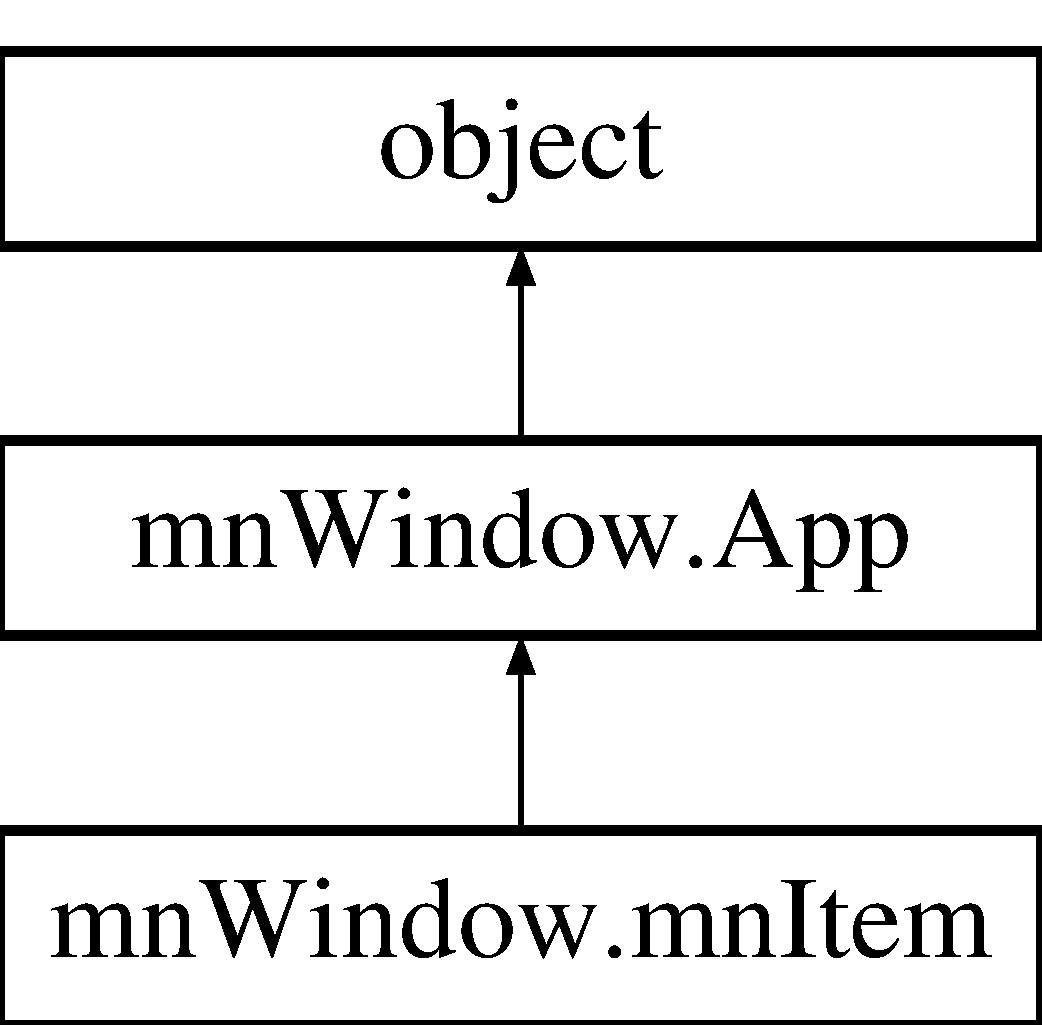
\includegraphics[height=3.000000cm]{d4/d8e/classmnWindow_1_1App}
\end{center}
\end{figure}
\subsection*{Veřejné metody}
\begin{DoxyCompactItemize}
\item 
def \hyperlink{classmnWindow_1_1App_ab0d57eebcf6c963177340604c8aa783a}{\-\_\-\-\_\-init\-\_\-\-\_\-}
\begin{DoxyCompactList}\small\item\em Constructor od the class. \end{DoxyCompactList}\item 
def \hyperlink{classmnWindow_1_1App_a0ae27dd2c076cc8bea3189d60c061a25}{start\-Listen}
\begin{DoxyCompactList}\small\item\em Method for starting listening to new media. \end{DoxyCompactList}\item 
def \hyperlink{classmnWindow_1_1App_a3224a0de9bd79c5213256b4da9e261ee}{list\-Res}
\begin{DoxyCompactList}\small\item\em Method for listing the dbase into window. \end{DoxyCompactList}\item 
def \hyperlink{classmnWindow_1_1App_a28eaa4c2614d33d923d97f7a365c4ec2}{key\-En}
\begin{DoxyCompactList}\small\item\em Method for enter in entry box for name. \end{DoxyCompactList}\item 
def \hyperlink{classmnWindow_1_1App_a9293245f3bbcd5eee738b923e948c281}{get\-List}
\begin{DoxyCompactList}\small\item\em Method for generating a list and calling txt reader from O\-S to show user. \end{DoxyCompactList}\item 
def \hyperlink{classmnWindow_1_1App_a7bd83a542a19260476e39415c73ff960}{key\-Nm}
\begin{DoxyCompactList}\small\item\em Method for enter in entry box for name. \end{DoxyCompactList}\item 
def \hyperlink{classmnWindow_1_1App_a4bd36c84cbc43fa9e27347ad7ec66ddd}{On\-Dub}
\begin{DoxyCompactList}\small\item\em Method for getting event from listbox. \end{DoxyCompactList}\item 
def \hyperlink{classmnWindow_1_1App_a3a711688d2463a65d43a0a9dcc19276c}{paint\-Layout}
\begin{DoxyCompactList}\small\item\em Method painting main window. \end{DoxyCompactList}\item 
def \hyperlink{classmnWindow_1_1App_aa07a9b47b0fc8969a970edff8ecc1b56}{load\-Progs}
\begin{DoxyCompactList}\small\item\em Method for progressbar changes and messages passing to user. \end{DoxyCompactList}\item 
def \hyperlink{classmnWindow_1_1App_a6db9e81dd9a0225e260c43852f6bdcc4}{qquit}
\begin{DoxyCompactList}\small\item\em Metoda pro ukončení okna Je nutné vypnout vlákno, které vykonává příkazy na pozadí okna. \end{DoxyCompactList}\end{DoxyCompactItemize}
\subsection*{Veřejné atributy}
\begin{DoxyCompactItemize}
\item 
\hypertarget{classmnWindow_1_1App_a9b8f027f874a31feb1e35ade7cab8d50}{\hyperlink{classmnWindow_1_1App_a9b8f027f874a31feb1e35ade7cab8d50}{root}}\label{classmnWindow_1_1App_a9b8f027f874a31feb1e35ade7cab8d50}

\begin{DoxyCompactList}\small\item\em Pointer on T\-K window. \end{DoxyCompactList}\item 
\hypertarget{classmnWindow_1_1App_a67b24743ac9fa2139f09eeee00165afe}{\hyperlink{classmnWindow_1_1App_a67b24743ac9fa2139f09eeee00165afe}{qi}}\label{classmnWindow_1_1App_a67b24743ac9fa2139f09eeee00165afe}

\begin{DoxyCompactList}\small\item\em Input quee. \end{DoxyCompactList}\item 
\hypertarget{classmnWindow_1_1App_a80bce5f82481df178a78c5658425ee01}{\hyperlink{classmnWindow_1_1App_a80bce5f82481df178a78c5658425ee01}{qo}}\label{classmnWindow_1_1App_a80bce5f82481df178a78c5658425ee01}

\begin{DoxyCompactList}\small\item\em Output quee. \end{DoxyCompactList}\item 
\hypertarget{classmnWindow_1_1App_ac3a59ee379070bd0b0c4c18d5e7daf8e}{\hyperlink{classmnWindow_1_1App_ac3a59ee379070bd0b0c4c18d5e7daf8e}{sysm}}\label{classmnWindow_1_1App_ac3a59ee379070bd0b0c4c18d5e7daf8e}

\begin{DoxyCompactList}\small\item\em Mounting sys class. \end{DoxyCompactList}\item 
\hypertarget{classmnWindow_1_1App_a40ee7c6ef712462b04cd33e7dbb5c73c}{\hyperlink{classmnWindow_1_1App_a40ee7c6ef712462b04cd33e7dbb5c73c}{db}}\label{classmnWindow_1_1App_a40ee7c6ef712462b04cd33e7dbb5c73c}

\begin{DoxyCompactList}\small\item\em D\-B handle. \end{DoxyCompactList}\item 
\hypertarget{classmnWindow_1_1App_af5c4a34cc9dbc91f97acfd87e95221de}{\hyperlink{classmnWindow_1_1App_af5c4a34cc9dbc91f97acfd87e95221de}{lo}}\label{classmnWindow_1_1App_af5c4a34cc9dbc91f97acfd87e95221de}

\begin{DoxyCompactList}\small\item\em New device detection activation. \end{DoxyCompactList}\item 
\hypertarget{classmnWindow_1_1App_a12abbfb4d033c684d65bb555d61b2d5a}{\hyperlink{classmnWindow_1_1App_a12abbfb4d033c684d65bb555d61b2d5a}{name}}\label{classmnWindow_1_1App_a12abbfb4d033c684d65bb555d61b2d5a}

\begin{DoxyCompactList}\small\item\em Name of currently loading devices. \end{DoxyCompactList}\item 
\hypertarget{classmnWindow_1_1App_af69811a5d0fe5a1c25c4b3dbda906dc3}{{\bfseries dvs}}\label{classmnWindow_1_1App_af69811a5d0fe5a1c25c4b3dbda906dc3}

\item 
\hypertarget{classmnWindow_1_1App_a1ecace680297abb30e0525f6336e6ad6}{\hyperlink{classmnWindow_1_1App_a1ecace680297abb30e0525f6336e6ad6}{beg}}\label{classmnWindow_1_1App_a1ecace680297abb30e0525f6336e6ad6}

\begin{DoxyCompactList}\small\item\em Beggining button. \end{DoxyCompactList}\item 
\hypertarget{classmnWindow_1_1App_aca1d00ea1052ac20f926348d4d5f73e4}{{\bfseries v}}\label{classmnWindow_1_1App_aca1d00ea1052ac20f926348d4d5f73e4}

\item 
\hypertarget{classmnWindow_1_1App_a2c4678ace0b9f4bbf7e0970914b32ab0}{\hyperlink{classmnWindow_1_1App_a2c4678ace0b9f4bbf7e0970914b32ab0}{ew}}\label{classmnWindow_1_1App_a2c4678ace0b9f4bbf7e0970914b32ab0}

\begin{DoxyCompactList}\small\item\em Var telling what to choose. \end{DoxyCompactList}\item 
\hypertarget{classmnWindow_1_1App_aa3bdf8ebe04fbd8731def76c830e4293}{\hyperlink{classmnWindow_1_1App_aa3bdf8ebe04fbd8731def76c830e4293}{tl}}\label{classmnWindow_1_1App_aa3bdf8ebe04fbd8731def76c830e4293}

\begin{DoxyCompactList}\small\item\em List of D\-B items. \end{DoxyCompactList}\item 
\hypertarget{classmnWindow_1_1App_aa13141f8175c2e7232b620272e953bc9}{{\bfseries en}}\label{classmnWindow_1_1App_aa13141f8175c2e7232b620272e953bc9}

\item 
\hypertarget{classmnWindow_1_1App_acd9c0b1e01d55d8f7a70098a383315e8}{\hyperlink{classmnWindow_1_1App_acd9c0b1e01d55d8f7a70098a383315e8}{to}}\label{classmnWindow_1_1App_acd9c0b1e01d55d8f7a70098a383315e8}

\begin{DoxyCompactList}\small\item\em List for user notification. \end{DoxyCompactList}\item 
\hypertarget{classmnWindow_1_1App_a9749727ad725c621508d5abc185da40c}{\hyperlink{classmnWindow_1_1App_a9749727ad725c621508d5abc185da40c}{progressbar}}\label{classmnWindow_1_1App_a9749727ad725c621508d5abc185da40c}

\begin{DoxyCompactList}\small\item\em Pointer on current progress. \end{DoxyCompactList}\end{DoxyCompactItemize}


\subsection{Detailní popis}
Class containing gui. 

\subsection{Dokumentace konstruktoru a destruktoru}
\hypertarget{classmnWindow_1_1App_ab0d57eebcf6c963177340604c8aa783a}{\index{mn\-Window\-::\-App@{mn\-Window\-::\-App}!\-\_\-\-\_\-init\-\_\-\-\_\-@{\-\_\-\-\_\-init\-\_\-\-\_\-}}
\index{\-\_\-\-\_\-init\-\_\-\-\_\-@{\-\_\-\-\_\-init\-\_\-\-\_\-}!mnWindow::App@{mn\-Window\-::\-App}}
\subsubsection[{\-\_\-\-\_\-init\-\_\-\-\_\-}]{\setlength{\rightskip}{0pt plus 5cm}def mn\-Window.\-App.\-\_\-\-\_\-init\-\_\-\-\_\- (
\begin{DoxyParamCaption}
\item[{}]{self, }
\item[{}]{r, }
\item[{}]{qii, }
\item[{}]{qoi}
\end{DoxyParamCaption}
)}}\label{classmnWindow_1_1App_ab0d57eebcf6c963177340604c8aa783a}


Constructor od the class. 


\begin{DoxyParams}{Parametry}
{\em self} & Pointer on class \\
\hline
{\em r} & Pointer on Tkinker window \\
\hline
\end{DoxyParams}


\subsection{Dokumentace k metodám}
\hypertarget{classmnWindow_1_1App_a9293245f3bbcd5eee738b923e948c281}{\index{mn\-Window\-::\-App@{mn\-Window\-::\-App}!get\-List@{get\-List}}
\index{get\-List@{get\-List}!mnWindow::App@{mn\-Window\-::\-App}}
\subsubsection[{get\-List}]{\setlength{\rightskip}{0pt plus 5cm}def mn\-Window.\-App.\-get\-List (
\begin{DoxyParamCaption}
\item[{}]{self}
\end{DoxyParamCaption}
)}}\label{classmnWindow_1_1App_a9293245f3bbcd5eee738b923e948c281}


Method for generating a list and calling txt reader from O\-S to show user. 


\begin{DoxyParams}{Parametry}
{\em self} & Pointer on class \\
\hline
\end{DoxyParams}
\hypertarget{classmnWindow_1_1App_a28eaa4c2614d33d923d97f7a365c4ec2}{\index{mn\-Window\-::\-App@{mn\-Window\-::\-App}!key\-En@{key\-En}}
\index{key\-En@{key\-En}!mnWindow::App@{mn\-Window\-::\-App}}
\subsubsection[{key\-En}]{\setlength{\rightskip}{0pt plus 5cm}def mn\-Window.\-App.\-key\-En (
\begin{DoxyParamCaption}
\item[{}]{self, }
\item[{}]{evt}
\end{DoxyParamCaption}
)}}\label{classmnWindow_1_1App_a28eaa4c2614d33d923d97f7a365c4ec2}


Method for enter in entry box for name. 


\begin{DoxyParams}{Parametry}
{\em self} & Pointer on class \\
\hline
{\em evt} & Sended event \\
\hline
\end{DoxyParams}
\hypertarget{classmnWindow_1_1App_a7bd83a542a19260476e39415c73ff960}{\index{mn\-Window\-::\-App@{mn\-Window\-::\-App}!key\-Nm@{key\-Nm}}
\index{key\-Nm@{key\-Nm}!mnWindow::App@{mn\-Window\-::\-App}}
\subsubsection[{key\-Nm}]{\setlength{\rightskip}{0pt plus 5cm}def mn\-Window.\-App.\-key\-Nm (
\begin{DoxyParamCaption}
\item[{}]{self, }
\item[{}]{evt}
\end{DoxyParamCaption}
)}}\label{classmnWindow_1_1App_a7bd83a542a19260476e39415c73ff960}


Method for enter in entry box for name. 


\begin{DoxyParams}{Parametry}
{\em self} & Pointer on class \\
\hline
{\em evt} & Sended event \\
\hline
\end{DoxyParams}
\hypertarget{classmnWindow_1_1App_a3224a0de9bd79c5213256b4da9e261ee}{\index{mn\-Window\-::\-App@{mn\-Window\-::\-App}!list\-Res@{list\-Res}}
\index{list\-Res@{list\-Res}!mnWindow::App@{mn\-Window\-::\-App}}
\subsubsection[{list\-Res}]{\setlength{\rightskip}{0pt plus 5cm}def mn\-Window.\-App.\-list\-Res (
\begin{DoxyParamCaption}
\item[{}]{self, }
\item[{}]{reg = {\ttfamily \char`\"{}$\ast$\char`\"{}}}
\end{DoxyParamCaption}
)}}\label{classmnWindow_1_1App_a3224a0de9bd79c5213256b4da9e261ee}


Method for listing the dbase into window. 


\begin{DoxyParams}{Parametry}
{\em self} & Pointer on class \\
\hline
{\em reg} & Regular expresion \\
\hline
\end{DoxyParams}
\hypertarget{classmnWindow_1_1App_aa07a9b47b0fc8969a970edff8ecc1b56}{\index{mn\-Window\-::\-App@{mn\-Window\-::\-App}!load\-Progs@{load\-Progs}}
\index{load\-Progs@{load\-Progs}!mnWindow::App@{mn\-Window\-::\-App}}
\subsubsection[{load\-Progs}]{\setlength{\rightskip}{0pt plus 5cm}def mn\-Window.\-App.\-load\-Progs (
\begin{DoxyParamCaption}
\item[{}]{self, }
\item[{}]{qc}
\end{DoxyParamCaption}
)}}\label{classmnWindow_1_1App_aa07a9b47b0fc8969a970edff8ecc1b56}


Method for progressbar changes and messages passing to user. 


\begin{DoxyParams}{Parametry}
{\em self} & Ukazatel na objekt \\
\hline
{\em qc} & Výstupní fronta \\
\hline
\end{DoxyParams}
\hypertarget{classmnWindow_1_1App_a4bd36c84cbc43fa9e27347ad7ec66ddd}{\index{mn\-Window\-::\-App@{mn\-Window\-::\-App}!On\-Dub@{On\-Dub}}
\index{On\-Dub@{On\-Dub}!mnWindow::App@{mn\-Window\-::\-App}}
\subsubsection[{On\-Dub}]{\setlength{\rightskip}{0pt plus 5cm}def mn\-Window.\-App.\-On\-Dub (
\begin{DoxyParamCaption}
\item[{}]{self, }
\item[{}]{event}
\end{DoxyParamCaption}
)}}\label{classmnWindow_1_1App_a4bd36c84cbc43fa9e27347ad7ec66ddd}


Method for getting event from listbox. 


\begin{DoxyParams}{Parametry}
{\em self} & Pointer on class \\
\hline
{\em evt} & Sended event \\
\hline
\end{DoxyParams}
\hypertarget{classmnWindow_1_1App_a3a711688d2463a65d43a0a9dcc19276c}{\index{mn\-Window\-::\-App@{mn\-Window\-::\-App}!paint\-Layout@{paint\-Layout}}
\index{paint\-Layout@{paint\-Layout}!mnWindow::App@{mn\-Window\-::\-App}}
\subsubsection[{paint\-Layout}]{\setlength{\rightskip}{0pt plus 5cm}def mn\-Window.\-App.\-paint\-Layout (
\begin{DoxyParamCaption}
\item[{}]{self}
\end{DoxyParamCaption}
)}}\label{classmnWindow_1_1App_a3a711688d2463a65d43a0a9dcc19276c}


Method painting main window. 


\begin{DoxyParams}{Parametry}
{\em self} & Pointer on class \\
\hline
\end{DoxyParams}
\hypertarget{classmnWindow_1_1App_a6db9e81dd9a0225e260c43852f6bdcc4}{\index{mn\-Window\-::\-App@{mn\-Window\-::\-App}!qquit@{qquit}}
\index{qquit@{qquit}!mnWindow::App@{mn\-Window\-::\-App}}
\subsubsection[{qquit}]{\setlength{\rightskip}{0pt plus 5cm}def mn\-Window.\-App.\-qquit (
\begin{DoxyParamCaption}
\item[{}]{self}
\end{DoxyParamCaption}
)}}\label{classmnWindow_1_1App_a6db9e81dd9a0225e260c43852f6bdcc4}


Metoda pro ukončení okna Je nutné vypnout vlákno, které vykonává příkazy na pozadí okna. 


\begin{DoxyParams}{Parametry}
{\em self} & Ukazatel na objekt \\
\hline
\end{DoxyParams}
\hypertarget{classmnWindow_1_1App_a0ae27dd2c076cc8bea3189d60c061a25}{\index{mn\-Window\-::\-App@{mn\-Window\-::\-App}!start\-Listen@{start\-Listen}}
\index{start\-Listen@{start\-Listen}!mnWindow::App@{mn\-Window\-::\-App}}
\subsubsection[{start\-Listen}]{\setlength{\rightskip}{0pt plus 5cm}def mn\-Window.\-App.\-start\-Listen (
\begin{DoxyParamCaption}
\item[{}]{self}
\end{DoxyParamCaption}
)}}\label{classmnWindow_1_1App_a0ae27dd2c076cc8bea3189d60c061a25}


Method for starting listening to new media. 


\begin{DoxyParams}{Parametry}
{\em self} & Pointer on class \\
\hline
\end{DoxyParams}


Dokumentace pro tuto třídu byla generována z následujícího souboru\-:\begin{DoxyCompactItemize}
\item 
\hyperlink{mnWindow_8py}{mn\-Window.\-py}\end{DoxyCompactItemize}

\hypertarget{classmain_1_1Chdir}{\section{Dokumentace třídy main.\-Chdir}
\label{classmain_1_1Chdir}\index{main.\-Chdir@{main.\-Chdir}}
}


Class for rewriting path.  


\subsection*{Veřejné metody}
\begin{DoxyCompactItemize}
\item 
def \hyperlink{classmain_1_1Chdir_ac7361f2ea260c83ed6b42a7047c80214}{\-\_\-\-\_\-init\-\_\-\-\_\-}
\begin{DoxyCompactList}\small\item\em Constructor of the class. \end{DoxyCompactList}\item 
def \hyperlink{classmain_1_1Chdir_add811e304912724c03da489a37cfe2d5}{\-\_\-\-\_\-del\-\_\-\-\_\-}
\begin{DoxyCompactList}\small\item\em Desctructor on class. \end{DoxyCompactList}\end{DoxyCompactItemize}
\subsection*{Veřejné atributy}
\begin{DoxyCompactItemize}
\item 
\hypertarget{classmain_1_1Chdir_a8fcc4e44e462eb780f7694ba60f226d9}{\hyperlink{classmain_1_1Chdir_a8fcc4e44e462eb780f7694ba60f226d9}{saved\-Path}}\label{classmain_1_1Chdir_a8fcc4e44e462eb780f7694ba60f226d9}

\begin{DoxyCompactList}\small\item\em Saved path. \end{DoxyCompactList}\end{DoxyCompactItemize}


\subsection{Detailní popis}
Class for rewriting path. 

\subsection{Dokumentace konstruktoru a destruktoru}
\hypertarget{classmain_1_1Chdir_ac7361f2ea260c83ed6b42a7047c80214}{\index{main\-::\-Chdir@{main\-::\-Chdir}!\-\_\-\-\_\-init\-\_\-\-\_\-@{\-\_\-\-\_\-init\-\_\-\-\_\-}}
\index{\-\_\-\-\_\-init\-\_\-\-\_\-@{\-\_\-\-\_\-init\-\_\-\-\_\-}!main::Chdir@{main\-::\-Chdir}}
\subsubsection[{\-\_\-\-\_\-init\-\_\-\-\_\-}]{\setlength{\rightskip}{0pt plus 5cm}def main.\-Chdir.\-\_\-\-\_\-init\-\_\-\-\_\- (
\begin{DoxyParamCaption}
\item[{}]{self, }
\item[{}]{new\-Path}
\end{DoxyParamCaption}
)}}\label{classmain_1_1Chdir_ac7361f2ea260c83ed6b42a7047c80214}


Constructor of the class. 


\begin{DoxyParams}{Parametry}
{\em self} & Pointer on class \\
\hline
{\em new\-Path} & New path \\
\hline
\end{DoxyParams}
\hypertarget{classmain_1_1Chdir_add811e304912724c03da489a37cfe2d5}{\index{main\-::\-Chdir@{main\-::\-Chdir}!\-\_\-\-\_\-del\-\_\-\-\_\-@{\-\_\-\-\_\-del\-\_\-\-\_\-}}
\index{\-\_\-\-\_\-del\-\_\-\-\_\-@{\-\_\-\-\_\-del\-\_\-\-\_\-}!main::Chdir@{main\-::\-Chdir}}
\subsubsection[{\-\_\-\-\_\-del\-\_\-\-\_\-}]{\setlength{\rightskip}{0pt plus 5cm}def main.\-Chdir.\-\_\-\-\_\-del\-\_\-\-\_\- (
\begin{DoxyParamCaption}
\item[{}]{self}
\end{DoxyParamCaption}
)}}\label{classmain_1_1Chdir_add811e304912724c03da489a37cfe2d5}


Desctructor on class. 


\begin{DoxyParams}{Parametry}
{\em self} & Pointer on class \\
\hline
\end{DoxyParams}


Dokumentace pro tuto třídu byla generována z následujícího souboru\-:\begin{DoxyCompactItemize}
\item 
\hyperlink{main_8py}{main.\-py}\end{DoxyCompactItemize}

\hypertarget{classDBHand_1_1DBHand}{\section{Dokumentace třídy D\-B\-Hand.\-D\-B\-Hand}
\label{classDBHand_1_1DBHand}\index{D\-B\-Hand.\-D\-B\-Hand@{D\-B\-Hand.\-D\-B\-Hand}}
}


Class for working with D\-Bfiles.  


\subsection*{Veřejné metody}
\begin{DoxyCompactItemize}
\item 
def \hyperlink{classDBHand_1_1DBHand_a1da352dfe2f9be2bcb8dbc77e39b0da6}{\-\_\-\-\_\-init\-\_\-\-\_\-}
\begin{DoxyCompactList}\small\item\em Constructor of the class. \end{DoxyCompactList}\item 
def \hyperlink{classDBHand_1_1DBHand_a07a9d7a56e3aad6a2fb055afd3016a05}{get\-Last\-Name}
\begin{DoxyCompactList}\small\item\em Method for getting last name. \end{DoxyCompactList}\item 
def \hyperlink{classDBHand_1_1DBHand_af89e646985e27bb33622fbcf3d984d0d}{get\-By\-Name}
\begin{DoxyCompactList}\small\item\em Getter by name. \end{DoxyCompactList}\item 
def \hyperlink{classDBHand_1_1DBHand_a8e5cad73cd8440972885d7c7ac0328e2}{get\-By\-Date}
\begin{DoxyCompactList}\small\item\em Getter by date. \end{DoxyCompactList}\item 
def \hyperlink{classDBHand_1_1DBHand_ac7b5609f896d7e3b9e59fca09c521396}{get\-By\-Hash}
\begin{DoxyCompactList}\small\item\em Getter from dbase by hash. \end{DoxyCompactList}\item 
def \hyperlink{classDBHand_1_1DBHand_aaba58e5004798661d7d3cb5566ad1a45}{get\-By\-Cont\-Fls}
\begin{DoxyCompactList}\small\item\em Constructor of the class. \end{DoxyCompactList}\item 
def \hyperlink{classDBHand_1_1DBHand_a102843d4ad41bcf04b55044e20cc7db2}{gen\-New\-Input}
\begin{DoxyCompactList}\small\item\em Inputs new line in D\-Base. \end{DoxyCompactList}\item 
def \hyperlink{classDBHand_1_1DBHand_ab7fabebb9aeaf8bcb236a64d5bd9d344}{err\-Input}
\begin{DoxyCompactList}\small\item\em Erase input by name. \end{DoxyCompactList}\item 
def \hyperlink{classDBHand_1_1DBHand_aa038194a09dd084c5c872238d9a03ff5}{gen\-Bookl}
\begin{DoxyCompactList}\small\item\em Generate Booklet. \end{DoxyCompactList}\item 
def \hyperlink{classDBHand_1_1DBHand_a0840cbf8e159fcbb1c3162e7ea4b2537}{get\-List}
\begin{DoxyCompactList}\small\item\em Give a list of D\-Base entries. \end{DoxyCompactList}\item 
def \hyperlink{classDBHand_1_1DBHand_a399c895359ec5a0bf451e47c4a4274b1}{build\-List\-Txt}
\begin{DoxyCompactList}\small\item\em Give a list of D\-Base entries. \end{DoxyCompactList}\end{DoxyCompactItemize}
\subsection*{Veřejné atributy}
\begin{DoxyCompactItemize}
\item 
\hypertarget{classDBHand_1_1DBHand_a9a2cff8d8862395801ab604f1570f971}{\hyperlink{classDBHand_1_1DBHand_a9a2cff8d8862395801ab604f1570f971}{dbs}}\label{classDBHand_1_1DBHand_a9a2cff8d8862395801ab604f1570f971}

\begin{DoxyCompactList}\small\item\em Dbs file path. \end{DoxyCompactList}\item 
\hypertarget{classDBHand_1_1DBHand_a43d2f414ba37b36069bf6020098911b1}{\hyperlink{classDBHand_1_1DBHand_a43d2f414ba37b36069bf6020098911b1}{lsts}}\label{classDBHand_1_1DBHand_a43d2f414ba37b36069bf6020098911b1}

\begin{DoxyCompactList}\small\item\em List files dir. \end{DoxyCompactList}\end{DoxyCompactItemize}


\subsection{Detailní popis}
Class for working with D\-Bfiles. 

\subsection{Dokumentace konstruktoru a destruktoru}
\hypertarget{classDBHand_1_1DBHand_a1da352dfe2f9be2bcb8dbc77e39b0da6}{\index{D\-B\-Hand\-::\-D\-B\-Hand@{D\-B\-Hand\-::\-D\-B\-Hand}!\-\_\-\-\_\-init\-\_\-\-\_\-@{\-\_\-\-\_\-init\-\_\-\-\_\-}}
\index{\-\_\-\-\_\-init\-\_\-\-\_\-@{\-\_\-\-\_\-init\-\_\-\-\_\-}!DBHand::DBHand@{D\-B\-Hand\-::\-D\-B\-Hand}}
\subsubsection[{\-\_\-\-\_\-init\-\_\-\-\_\-}]{\setlength{\rightskip}{0pt plus 5cm}def D\-B\-Hand.\-D\-B\-Hand.\-\_\-\-\_\-init\-\_\-\-\_\- (
\begin{DoxyParamCaption}
\item[{}]{self}
\end{DoxyParamCaption}
)}}\label{classDBHand_1_1DBHand_a1da352dfe2f9be2bcb8dbc77e39b0da6}


Constructor of the class. 


\begin{DoxyParams}{Parametry}
{\em self} & Pointer on class \\
\hline
\end{DoxyParams}


\subsection{Dokumentace k metodám}
\hypertarget{classDBHand_1_1DBHand_a399c895359ec5a0bf451e47c4a4274b1}{\index{D\-B\-Hand\-::\-D\-B\-Hand@{D\-B\-Hand\-::\-D\-B\-Hand}!build\-List\-Txt@{build\-List\-Txt}}
\index{build\-List\-Txt@{build\-List\-Txt}!DBHand::DBHand@{D\-B\-Hand\-::\-D\-B\-Hand}}
\subsubsection[{build\-List\-Txt}]{\setlength{\rightskip}{0pt plus 5cm}def D\-B\-Hand.\-D\-B\-Hand.\-build\-List\-Txt (
\begin{DoxyParamCaption}
\item[{}]{self, }
\item[{}]{path = {\ttfamily \char`\"{}./list.txt\char`\"{}}}
\end{DoxyParamCaption}
)}}\label{classDBHand_1_1DBHand_a399c895359ec5a0bf451e47c4a4274b1}


Give a list of D\-Base entries. 


\begin{DoxyParams}{Parametry}
{\em path} & Name of output file to print a list \\
\hline
{\em self} & Pointer on class \\
\hline
\end{DoxyParams}
\hypertarget{classDBHand_1_1DBHand_ab7fabebb9aeaf8bcb236a64d5bd9d344}{\index{D\-B\-Hand\-::\-D\-B\-Hand@{D\-B\-Hand\-::\-D\-B\-Hand}!err\-Input@{err\-Input}}
\index{err\-Input@{err\-Input}!DBHand::DBHand@{D\-B\-Hand\-::\-D\-B\-Hand}}
\subsubsection[{err\-Input}]{\setlength{\rightskip}{0pt plus 5cm}def D\-B\-Hand.\-D\-B\-Hand.\-err\-Input (
\begin{DoxyParamCaption}
\item[{}]{self, }
\item[{}]{name}
\end{DoxyParamCaption}
)}}\label{classDBHand_1_1DBHand_ab7fabebb9aeaf8bcb236a64d5bd9d344}


Erase input by name. 


\begin{DoxyParams}{Parametry}
{\em name} & Name of media generated by appliacation \\
\hline
{\em self} & Pointer on class \\
\hline
\end{DoxyParams}
\hypertarget{classDBHand_1_1DBHand_aa038194a09dd084c5c872238d9a03ff5}{\index{D\-B\-Hand\-::\-D\-B\-Hand@{D\-B\-Hand\-::\-D\-B\-Hand}!gen\-Bookl@{gen\-Bookl}}
\index{gen\-Bookl@{gen\-Bookl}!DBHand::DBHand@{D\-B\-Hand\-::\-D\-B\-Hand}}
\subsubsection[{gen\-Bookl}]{\setlength{\rightskip}{0pt plus 5cm}def D\-B\-Hand.\-D\-B\-Hand.\-gen\-Bookl (
\begin{DoxyParamCaption}
\item[{}]{self, }
\item[{}]{li}
\end{DoxyParamCaption}
)}}\label{classDBHand_1_1DBHand_aa038194a09dd084c5c872238d9a03ff5}


Generate Booklet. 


\begin{DoxyParams}{Parametry}
{\em hash} & Id of item in db \\
\hline
{\em self} & Pointer on class \\
\hline
\end{DoxyParams}
\hypertarget{classDBHand_1_1DBHand_a102843d4ad41bcf04b55044e20cc7db2}{\index{D\-B\-Hand\-::\-D\-B\-Hand@{D\-B\-Hand\-::\-D\-B\-Hand}!gen\-New\-Input@{gen\-New\-Input}}
\index{gen\-New\-Input@{gen\-New\-Input}!DBHand::DBHand@{D\-B\-Hand\-::\-D\-B\-Hand}}
\subsubsection[{gen\-New\-Input}]{\setlength{\rightskip}{0pt plus 5cm}def D\-B\-Hand.\-D\-B\-Hand.\-gen\-New\-Input (
\begin{DoxyParamCaption}
\item[{}]{self, }
\item[{}]{name, }
\item[{}]{fl\-P, }
\item[{}]{mnt, }
\item[{}]{qo = {\ttfamily None}}
\end{DoxyParamCaption}
)}}\label{classDBHand_1_1DBHand_a102843d4ad41bcf04b55044e20cc7db2}


Inputs new line in D\-Base. 


\begin{DoxyParams}{Parametry}
{\em name} & Name of media given by user \\
\hline
{\em mnt} & Mounted fs \\
\hline
{\em self} & Pointer on class \\
\hline
\end{DoxyParams}
\hypertarget{classDBHand_1_1DBHand_aaba58e5004798661d7d3cb5566ad1a45}{\index{D\-B\-Hand\-::\-D\-B\-Hand@{D\-B\-Hand\-::\-D\-B\-Hand}!get\-By\-Cont\-Fls@{get\-By\-Cont\-Fls}}
\index{get\-By\-Cont\-Fls@{get\-By\-Cont\-Fls}!DBHand::DBHand@{D\-B\-Hand\-::\-D\-B\-Hand}}
\subsubsection[{get\-By\-Cont\-Fls}]{\setlength{\rightskip}{0pt plus 5cm}def D\-B\-Hand.\-D\-B\-Hand.\-get\-By\-Cont\-Fls (
\begin{DoxyParamCaption}
\item[{}]{self, }
\item[{}]{name}
\end{DoxyParamCaption}
)}}\label{classDBHand_1_1DBHand_aaba58e5004798661d7d3cb5566ad1a45}


Constructor of the class. 


\begin{DoxyParams}{Parametry}
{\em name} & Name of file to by looking \\
\hline
{\em self} & Pointer on class \\
\hline
\end{DoxyParams}
\begin{DoxyReturn}{Návratová hodnota}
Dict containing result 
\end{DoxyReturn}
\hypertarget{classDBHand_1_1DBHand_a8e5cad73cd8440972885d7c7ac0328e2}{\index{D\-B\-Hand\-::\-D\-B\-Hand@{D\-B\-Hand\-::\-D\-B\-Hand}!get\-By\-Date@{get\-By\-Date}}
\index{get\-By\-Date@{get\-By\-Date}!DBHand::DBHand@{D\-B\-Hand\-::\-D\-B\-Hand}}
\subsubsection[{get\-By\-Date}]{\setlength{\rightskip}{0pt plus 5cm}def D\-B\-Hand.\-D\-B\-Hand.\-get\-By\-Date (
\begin{DoxyParamCaption}
\item[{}]{self, }
\item[{}]{date}
\end{DoxyParamCaption}
)}}\label{classDBHand_1_1DBHand_a8e5cad73cd8440972885d7c7ac0328e2}


Getter by date. 


\begin{DoxyParams}{Parametry}
{\em name} & Name of medium \\
\hline
{\em self} & Pointer on class \\
\hline
\end{DoxyParams}
\begin{DoxyReturn}{Návratová hodnota}
Dict containing result 
\end{DoxyReturn}
\hypertarget{classDBHand_1_1DBHand_ac7b5609f896d7e3b9e59fca09c521396}{\index{D\-B\-Hand\-::\-D\-B\-Hand@{D\-B\-Hand\-::\-D\-B\-Hand}!get\-By\-Hash@{get\-By\-Hash}}
\index{get\-By\-Hash@{get\-By\-Hash}!DBHand::DBHand@{D\-B\-Hand\-::\-D\-B\-Hand}}
\subsubsection[{get\-By\-Hash}]{\setlength{\rightskip}{0pt plus 5cm}def D\-B\-Hand.\-D\-B\-Hand.\-get\-By\-Hash (
\begin{DoxyParamCaption}
\item[{}]{self, }
\item[{}]{hash}
\end{DoxyParamCaption}
)}}\label{classDBHand_1_1DBHand_ac7b5609f896d7e3b9e59fca09c521396}


Getter from dbase by hash. 


\begin{DoxyParams}{Parametry}
{\em hash} & Hash of medium \\
\hline
{\em self} & Pointer on class \\
\hline
\end{DoxyParams}
\begin{DoxyReturn}{Návratová hodnota}
Dict containing result 
\end{DoxyReturn}
\hypertarget{classDBHand_1_1DBHand_af89e646985e27bb33622fbcf3d984d0d}{\index{D\-B\-Hand\-::\-D\-B\-Hand@{D\-B\-Hand\-::\-D\-B\-Hand}!get\-By\-Name@{get\-By\-Name}}
\index{get\-By\-Name@{get\-By\-Name}!DBHand::DBHand@{D\-B\-Hand\-::\-D\-B\-Hand}}
\subsubsection[{get\-By\-Name}]{\setlength{\rightskip}{0pt plus 5cm}def D\-B\-Hand.\-D\-B\-Hand.\-get\-By\-Name (
\begin{DoxyParamCaption}
\item[{}]{self, }
\item[{}]{name}
\end{DoxyParamCaption}
)}}\label{classDBHand_1_1DBHand_af89e646985e27bb33622fbcf3d984d0d}


Getter by name. 


\begin{DoxyParams}{Parametry}
{\em name} & Name of medium \\
\hline
{\em self} & Pointer on class \\
\hline
\end{DoxyParams}
\begin{DoxyReturn}{Návratová hodnota}
Dict containing result 
\end{DoxyReturn}
\hypertarget{classDBHand_1_1DBHand_a07a9d7a56e3aad6a2fb055afd3016a05}{\index{D\-B\-Hand\-::\-D\-B\-Hand@{D\-B\-Hand\-::\-D\-B\-Hand}!get\-Last\-Name@{get\-Last\-Name}}
\index{get\-Last\-Name@{get\-Last\-Name}!DBHand::DBHand@{D\-B\-Hand\-::\-D\-B\-Hand}}
\subsubsection[{get\-Last\-Name}]{\setlength{\rightskip}{0pt plus 5cm}def D\-B\-Hand.\-D\-B\-Hand.\-get\-Last\-Name (
\begin{DoxyParamCaption}
\item[{}]{self}
\end{DoxyParamCaption}
)}}\label{classDBHand_1_1DBHand_a07a9d7a56e3aad6a2fb055afd3016a05}


Method for getting last name. 


\begin{DoxyParams}{Parametry}
{\em self} & Pointer on class \\
\hline
\end{DoxyParams}
\begin{DoxyReturn}{Návratová hodnota}
Last name 
\end{DoxyReturn}
\hypertarget{classDBHand_1_1DBHand_a0840cbf8e159fcbb1c3162e7ea4b2537}{\index{D\-B\-Hand\-::\-D\-B\-Hand@{D\-B\-Hand\-::\-D\-B\-Hand}!get\-List@{get\-List}}
\index{get\-List@{get\-List}!DBHand::DBHand@{D\-B\-Hand\-::\-D\-B\-Hand}}
\subsubsection[{get\-List}]{\setlength{\rightskip}{0pt plus 5cm}def D\-B\-Hand.\-D\-B\-Hand.\-get\-List (
\begin{DoxyParamCaption}
\item[{}]{self}
\end{DoxyParamCaption}
)}}\label{classDBHand_1_1DBHand_a0840cbf8e159fcbb1c3162e7ea4b2537}


Give a list of D\-Base entries. 


\begin{DoxyParams}{Parametry}
{\em self} & Pointer on class \\
\hline
\end{DoxyParams}


Dokumentace pro tuto třídu byla generována z následujícího souboru\-:\begin{DoxyCompactItemize}
\item 
\hyperlink{DBHand_8py}{D\-B\-Hand.\-py}\end{DoxyCompactItemize}

\hypertarget{classIndx_1_1Indx}{\section{Dokumentace třídy Indx.\-Indx}
\label{classIndx_1_1Indx}\index{Indx.\-Indx@{Indx.\-Indx}}
}


Class for indexing and information selecting.  


\subsection*{Veřejné metody}
\begin{DoxyCompactItemize}
\item 
def \hyperlink{classIndx_1_1Indx_ae470547083e5bb49949c3a2578af4140}{hash\-File}
\begin{DoxyCompactList}\small\item\em Method for file hashing. \end{DoxyCompactList}\item 
def \hyperlink{classIndx_1_1Indx_a4b7a4ce268afe5074da5e82d1f8eb606}{make\-Name}
\begin{DoxyCompactList}\small\item\em Method for generating name of file. \end{DoxyCompactList}\item 
def \hyperlink{classIndx_1_1Indx_a462f189faaca04aec8b10b04d12ca885}{get\-Time}
\begin{DoxyCompactList}\small\item\em Method for generating timestamp. \end{DoxyCompactList}\item 
def \hyperlink{classIndx_1_1Indx_a9944c7978590e48746130415cd919895}{lst\-Files}
\begin{DoxyCompactList}\small\item\em Method for generating list of files in medium. \end{DoxyCompactList}\end{DoxyCompactItemize}


\subsection{Detailní popis}
Class for indexing and information selecting. 

\subsection{Dokumentace k metodám}
\hypertarget{classIndx_1_1Indx_a462f189faaca04aec8b10b04d12ca885}{\index{Indx\-::\-Indx@{Indx\-::\-Indx}!get\-Time@{get\-Time}}
\index{get\-Time@{get\-Time}!Indx::Indx@{Indx\-::\-Indx}}
\subsubsection[{get\-Time}]{\setlength{\rightskip}{0pt plus 5cm}def Indx.\-Indx.\-get\-Time (
\begin{DoxyParamCaption}
\item[{}]{self, }
\item[{}]{timestp = {\ttfamily \char`\"{}\mbox{[}\%H\-:\%M\-:\%S~\%d.\%m.\%Y\mbox{]}\char`\"{}}}
\end{DoxyParamCaption}
)}}\label{classIndx_1_1Indx_a462f189faaca04aec8b10b04d12ca885}


Method for generating timestamp. 


\begin{DoxyParams}{Parametry}
{\em self} & Pointer on class \\
\hline
{\em timestp} & Timestamp \\
\hline
\end{DoxyParams}
\begin{DoxyReturn}{Návratová hodnota}
String containing timestamp 
\end{DoxyReturn}
\hypertarget{classIndx_1_1Indx_ae470547083e5bb49949c3a2578af4140}{\index{Indx\-::\-Indx@{Indx\-::\-Indx}!hash\-File@{hash\-File}}
\index{hash\-File@{hash\-File}!Indx::Indx@{Indx\-::\-Indx}}
\subsubsection[{hash\-File}]{\setlength{\rightskip}{0pt plus 5cm}def Indx.\-Indx.\-hash\-File (
\begin{DoxyParamCaption}
\item[{}]{self, }
\item[{}]{name}
\end{DoxyParamCaption}
)}}\label{classIndx_1_1Indx_ae470547083e5bb49949c3a2578af4140}


Method for file hashing. 


\begin{DoxyParams}{Parametry}
{\em self} & Pointer on class \\
\hline
{\em name} & Name path to hashed file \\
\hline
\end{DoxyParams}
\begin{DoxyReturn}{Návratová hodnota}
String containing hash of file 
\end{DoxyReturn}
\hypertarget{classIndx_1_1Indx_a9944c7978590e48746130415cd919895}{\index{Indx\-::\-Indx@{Indx\-::\-Indx}!lst\-Files@{lst\-Files}}
\index{lst\-Files@{lst\-Files}!Indx::Indx@{Indx\-::\-Indx}}
\subsubsection[{lst\-Files}]{\setlength{\rightskip}{0pt plus 5cm}def Indx.\-Indx.\-lst\-Files (
\begin{DoxyParamCaption}
\item[{}]{self, }
\item[{}]{path = {\ttfamily \char`\"{}\char`\"{}}}
\end{DoxyParamCaption}
)}}\label{classIndx_1_1Indx_a9944c7978590e48746130415cd919895}


Method for generating list of files in medium. 


\begin{DoxyParams}{Parametry}
{\em self} & Pointer on class \\
\hline
{\em path} & Path to listing file \\
\hline
\end{DoxyParams}
\begin{DoxyReturn}{Návratová hodnota}
List of files 
\end{DoxyReturn}
\hypertarget{classIndx_1_1Indx_a4b7a4ce268afe5074da5e82d1f8eb606}{\index{Indx\-::\-Indx@{Indx\-::\-Indx}!make\-Name@{make\-Name}}
\index{make\-Name@{make\-Name}!Indx::Indx@{Indx\-::\-Indx}}
\subsubsection[{make\-Name}]{\setlength{\rightskip}{0pt plus 5cm}def Indx.\-Indx.\-make\-Name (
\begin{DoxyParamCaption}
\item[{}]{self, }
\item[{}]{name = {\ttfamily \char`\"{}\char`\"{}}, }
\item[{}]{db = {\ttfamily None}}
\end{DoxyParamCaption}
)}}\label{classIndx_1_1Indx_a4b7a4ce268afe5074da5e82d1f8eb606}


Method for generating name of file. 


\begin{DoxyParams}{Parametry}
{\em self} & Pointer on class \\
\hline
{\em name} & Name path to hashed file \\
\hline
\end{DoxyParams}
\begin{DoxyReturn}{Návratová hodnota}
String containing name of new medium 
\end{DoxyReturn}


Dokumentace pro tuto třídu byla generována z následujícího souboru\-:\begin{DoxyCompactItemize}
\item 
\hyperlink{Indx_8py}{Indx.\-py}\end{DoxyCompactItemize}

\hypertarget{classmnWindow_1_1mnItem}{\section{Dokumentace třídy mn\-Window.\-mn\-Item}
\label{classmnWindow_1_1mnItem}\index{mn\-Window.\-mn\-Item@{mn\-Window.\-mn\-Item}}
}


Class containing gui for selected item.  


Diagram dědičnosti pro třídu mn\-Window.\-mn\-Item\begin{figure}[H]
\begin{center}
\leavevmode
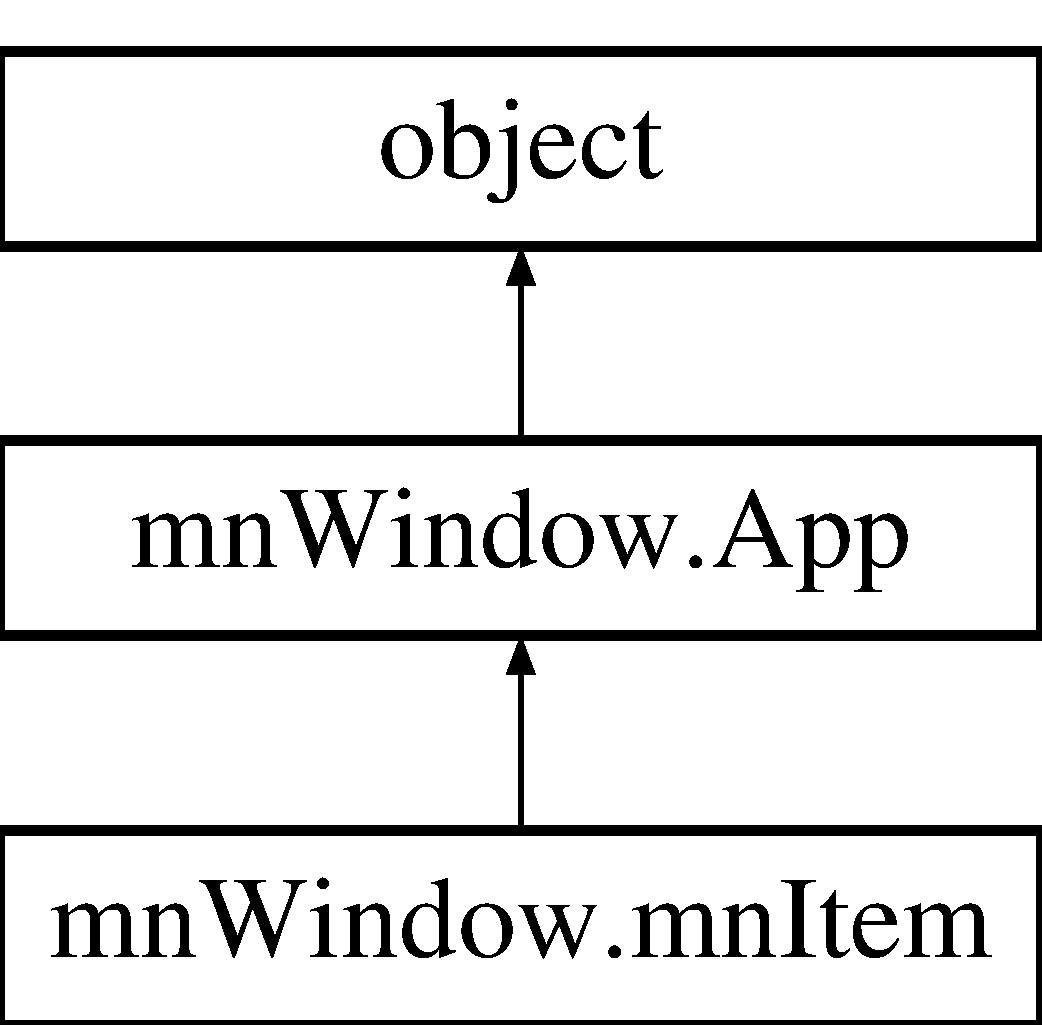
\includegraphics[height=3.000000cm]{db/dee/classmnWindow_1_1mnItem}
\end{center}
\end{figure}
\subsection*{Veřejné metody}
\begin{DoxyCompactItemize}
\item 
def \hyperlink{classmnWindow_1_1mnItem_af01fc782be86642d4108ef8bd83fdf75}{\-\_\-\-\_\-init\-\_\-\-\_\-}
\begin{DoxyCompactList}\small\item\em Constructor of window. \end{DoxyCompactList}\item 
def \hyperlink{classmnWindow_1_1mnItem_a9af6ba5f9bdfd604cf8e415fcb2ccf7f}{get\-Book}
\begin{DoxyCompactList}\small\item\em Booklet opener. \end{DoxyCompactList}\item 
def \hyperlink{classmnWindow_1_1mnItem_ae53c84d4ee29e3dc504b144224179aef}{err\-Item}
\begin{DoxyCompactList}\small\item\em Method for erasing item. \end{DoxyCompactList}\item 
def \hyperlink{classmnWindow_1_1mnItem_aa3d189e9da59ad27dcde5fba34f4fe8f}{paint\-Layout}
\begin{DoxyCompactList}\small\item\em Method painting main window. \end{DoxyCompactList}\end{DoxyCompactItemize}
\subsection*{Veřejné atributy}
\begin{DoxyCompactItemize}
\item 
\hypertarget{classmnWindow_1_1mnItem_a6938c30770e4a044a762888597d08f5f}{\hyperlink{classmnWindow_1_1mnItem_a6938c30770e4a044a762888597d08f5f}{app}}\label{classmnWindow_1_1mnItem_a6938c30770e4a044a762888597d08f5f}

\begin{DoxyCompactList}\small\item\em Instance of upper window. \end{DoxyCompactList}\item 
\hypertarget{classmnWindow_1_1mnItem_ad9c3fb1fd3637cc505dc8e03c0d4b7dd}{\hyperlink{classmnWindow_1_1mnItem_ad9c3fb1fd3637cc505dc8e03c0d4b7dd}{ls}}\label{classmnWindow_1_1mnItem_ad9c3fb1fd3637cc505dc8e03c0d4b7dd}

\begin{DoxyCompactList}\small\item\em Item from database. \end{DoxyCompactList}\item 
\hypertarget{classmnWindow_1_1mnItem_aadaa7063be7f422fad9f9282d01c7209}{\hyperlink{classmnWindow_1_1mnItem_aadaa7063be7f422fad9f9282d01c7209}{root}}\label{classmnWindow_1_1mnItem_aadaa7063be7f422fad9f9282d01c7209}

\begin{DoxyCompactList}\small\item\em Pointer on T\-K window. \end{DoxyCompactList}\item 
\hypertarget{classmnWindow_1_1mnItem_aca705dc598d43c6fedeeae7492157f3f}{\hyperlink{classmnWindow_1_1mnItem_aca705dc598d43c6fedeeae7492157f3f}{db}}\label{classmnWindow_1_1mnItem_aca705dc598d43c6fedeeae7492157f3f}

\begin{DoxyCompactList}\small\item\em Pointer on D\-Base. \end{DoxyCompactList}\end{DoxyCompactItemize}


\subsection{Detailní popis}
Class containing gui for selected item. 

\subsection{Dokumentace konstruktoru a destruktoru}
\hypertarget{classmnWindow_1_1mnItem_af01fc782be86642d4108ef8bd83fdf75}{\index{mn\-Window\-::mn\-Item@{mn\-Window\-::mn\-Item}!\-\_\-\-\_\-init\-\_\-\-\_\-@{\-\_\-\-\_\-init\-\_\-\-\_\-}}
\index{\-\_\-\-\_\-init\-\_\-\-\_\-@{\-\_\-\-\_\-init\-\_\-\-\_\-}!mnWindow::mnItem@{mn\-Window\-::mn\-Item}}
\subsubsection[{\-\_\-\-\_\-init\-\_\-\-\_\-}]{\setlength{\rightskip}{0pt plus 5cm}def mn\-Window.\-mn\-Item.\-\_\-\-\_\-init\-\_\-\-\_\- (
\begin{DoxyParamCaption}
\item[{}]{self, }
\item[{}]{win, }
\item[{}]{ls, }
\item[{}]{app}
\end{DoxyParamCaption}
)}}\label{classmnWindow_1_1mnItem_af01fc782be86642d4108ef8bd83fdf75}


Constructor of window. 


\begin{DoxyParams}{Parametry}
{\em self} & Pointer on class \\
\hline
{\em win} & Pointer on Tkinker window \\
\hline
{\em ls} & Item in D\-B \\
\hline
{\em app} & Upper instance of window \\
\hline
\end{DoxyParams}


\subsection{Dokumentace k metodám}
\hypertarget{classmnWindow_1_1mnItem_ae53c84d4ee29e3dc504b144224179aef}{\index{mn\-Window\-::mn\-Item@{mn\-Window\-::mn\-Item}!err\-Item@{err\-Item}}
\index{err\-Item@{err\-Item}!mnWindow::mnItem@{mn\-Window\-::mn\-Item}}
\subsubsection[{err\-Item}]{\setlength{\rightskip}{0pt plus 5cm}def mn\-Window.\-mn\-Item.\-err\-Item (
\begin{DoxyParamCaption}
\item[{}]{self}
\end{DoxyParamCaption}
)}}\label{classmnWindow_1_1mnItem_ae53c84d4ee29e3dc504b144224179aef}


Method for erasing item. 


\begin{DoxyParams}{Parametry}
{\em self} & Pointer on class \\
\hline
\end{DoxyParams}
\hypertarget{classmnWindow_1_1mnItem_a9af6ba5f9bdfd604cf8e415fcb2ccf7f}{\index{mn\-Window\-::mn\-Item@{mn\-Window\-::mn\-Item}!get\-Book@{get\-Book}}
\index{get\-Book@{get\-Book}!mnWindow::mnItem@{mn\-Window\-::mn\-Item}}
\subsubsection[{get\-Book}]{\setlength{\rightskip}{0pt plus 5cm}def mn\-Window.\-mn\-Item.\-get\-Book (
\begin{DoxyParamCaption}
\item[{}]{self}
\end{DoxyParamCaption}
)}}\label{classmnWindow_1_1mnItem_a9af6ba5f9bdfd604cf8e415fcb2ccf7f}


Booklet opener. 


\begin{DoxyParams}{Parametry}
{\em self} & Pointer on class \\
\hline
\end{DoxyParams}
\hypertarget{classmnWindow_1_1mnItem_aa3d189e9da59ad27dcde5fba34f4fe8f}{\index{mn\-Window\-::mn\-Item@{mn\-Window\-::mn\-Item}!paint\-Layout@{paint\-Layout}}
\index{paint\-Layout@{paint\-Layout}!mnWindow::mnItem@{mn\-Window\-::mn\-Item}}
\subsubsection[{paint\-Layout}]{\setlength{\rightskip}{0pt plus 5cm}def mn\-Window.\-mn\-Item.\-paint\-Layout (
\begin{DoxyParamCaption}
\item[{}]{self}
\end{DoxyParamCaption}
)}}\label{classmnWindow_1_1mnItem_aa3d189e9da59ad27dcde5fba34f4fe8f}


Method painting main window. 


\begin{DoxyParams}{Parametry}
{\em self} & Pointer on class \\
\hline
\end{DoxyParams}


Dokumentace pro tuto třídu byla generována z následujícího souboru\-:\begin{DoxyCompactItemize}
\item 
\hyperlink{mnWindow_8py}{mn\-Window.\-py}\end{DoxyCompactItemize}

\hypertarget{classSysMnt_1_1SysMnt}{\section{Dokumentace třídy Sys\-Mnt.\-Sys\-Mnt}
\label{classSysMnt_1_1SysMnt}\index{Sys\-Mnt.\-Sys\-Mnt@{Sys\-Mnt.\-Sys\-Mnt}}
}


Class containing methods for mounting/listing devices.  


\subsection*{Veřejné metody}
\begin{DoxyCompactItemize}
\item 
\hypertarget{classSysMnt_1_1SysMnt_ae5cf3574dd0a7508c9d84184dccf55f1}{def {\bfseries is\-\_\-block\-\_\-device}}\label{classSysMnt_1_1SysMnt_ae5cf3574dd0a7508c9d84184dccf55f1}

\item 
def \hyperlink{classSysMnt_1_1SysMnt_a5e4cb1666ae4827b9824b11b0fabbadf}{get\-List}
\begin{DoxyCompactList}\small\item\em Method to get list of block devices. \end{DoxyCompactList}\item 
def \hyperlink{classSysMnt_1_1SysMnt_a3fab8f0e7fa379fe5a416d9a962d0870}{tst\-Mount}
\begin{DoxyCompactList}\small\item\em Method to mount device. \end{DoxyCompactList}\item 
def \hyperlink{classSysMnt_1_1SysMnt_a0d75f68939cb5bb90aca5f5fc480c81e}{dd\-Sam}
\begin{DoxyCompactList}\small\item\em Method to create sample of block file. \end{DoxyCompactList}\item 
def \hyperlink{classSysMnt_1_1SysMnt_ab060ce00b125e74ab01c872c95ffb3f1}{u\-Mnt}
\begin{DoxyCompactList}\small\item\em Method to umount. \end{DoxyCompactList}\end{DoxyCompactItemize}


\subsection{Detailní popis}
Class containing methods for mounting/listing devices. 

\subsection{Dokumentace k metodám}
\hypertarget{classSysMnt_1_1SysMnt_a0d75f68939cb5bb90aca5f5fc480c81e}{\index{Sys\-Mnt\-::\-Sys\-Mnt@{Sys\-Mnt\-::\-Sys\-Mnt}!dd\-Sam@{dd\-Sam}}
\index{dd\-Sam@{dd\-Sam}!SysMnt::SysMnt@{Sys\-Mnt\-::\-Sys\-Mnt}}
\subsubsection[{dd\-Sam}]{\setlength{\rightskip}{0pt plus 5cm}def Sys\-Mnt.\-Sys\-Mnt.\-dd\-Sam (
\begin{DoxyParamCaption}
\item[{}]{self, }
\item[{}]{name, }
\item[{}]{size = {\ttfamily 100}}
\end{DoxyParamCaption}
)}}\label{classSysMnt_1_1SysMnt_a0d75f68939cb5bb90aca5f5fc480c81e}


Method to create sample of block file. 


\begin{DoxyParams}{Parametry}
{\em name} & Name of file \\
\hline
{\em size} & Size of file in M\-B \\
\hline
{\em self} & Point on class \\
\hline
\end{DoxyParams}
\hypertarget{classSysMnt_1_1SysMnt_a5e4cb1666ae4827b9824b11b0fabbadf}{\index{Sys\-Mnt\-::\-Sys\-Mnt@{Sys\-Mnt\-::\-Sys\-Mnt}!get\-List@{get\-List}}
\index{get\-List@{get\-List}!SysMnt::SysMnt@{Sys\-Mnt\-::\-Sys\-Mnt}}
\subsubsection[{get\-List}]{\setlength{\rightskip}{0pt plus 5cm}def Sys\-Mnt.\-Sys\-Mnt.\-get\-List (
\begin{DoxyParamCaption}
\item[{}]{self}
\end{DoxyParamCaption}
)}}\label{classSysMnt_1_1SysMnt_a5e4cb1666ae4827b9824b11b0fabbadf}


Method to get list of block devices. 


\begin{DoxyParams}{Parametry}
{\em self} & Point on class \\
\hline
\end{DoxyParams}
\begin{DoxyReturn}{Návratová hodnota}
List of block devices 
\end{DoxyReturn}
\hypertarget{classSysMnt_1_1SysMnt_a3fab8f0e7fa379fe5a416d9a962d0870}{\index{Sys\-Mnt\-::\-Sys\-Mnt@{Sys\-Mnt\-::\-Sys\-Mnt}!tst\-Mount@{tst\-Mount}}
\index{tst\-Mount@{tst\-Mount}!SysMnt::SysMnt@{Sys\-Mnt\-::\-Sys\-Mnt}}
\subsubsection[{tst\-Mount}]{\setlength{\rightskip}{0pt plus 5cm}def Sys\-Mnt.\-Sys\-Mnt.\-tst\-Mount (
\begin{DoxyParamCaption}
\item[{}]{self, }
\item[{}]{name}
\end{DoxyParamCaption}
)}}\label{classSysMnt_1_1SysMnt_a3fab8f0e7fa379fe5a416d9a962d0870}


Method to mount device. 


\begin{DoxyParams}{Parametry}
{\em name} & Device to be mounted \\
\hline
{\em self} & Point on class \\
\hline
\end{DoxyParams}
\begin{DoxyReturn}{Návratová hodnota}
True if mounted, false if it failed 
\end{DoxyReturn}
\hypertarget{classSysMnt_1_1SysMnt_ab060ce00b125e74ab01c872c95ffb3f1}{\index{Sys\-Mnt\-::\-Sys\-Mnt@{Sys\-Mnt\-::\-Sys\-Mnt}!u\-Mnt@{u\-Mnt}}
\index{u\-Mnt@{u\-Mnt}!SysMnt::SysMnt@{Sys\-Mnt\-::\-Sys\-Mnt}}
\subsubsection[{u\-Mnt}]{\setlength{\rightskip}{0pt plus 5cm}def Sys\-Mnt.\-Sys\-Mnt.\-u\-Mnt (
\begin{DoxyParamCaption}
\item[{}]{self}
\end{DoxyParamCaption}
)}}\label{classSysMnt_1_1SysMnt_ab060ce00b125e74ab01c872c95ffb3f1}


Method to umount. 


\begin{DoxyParams}{Parametry}
{\em self} & Point on class \\
\hline
\end{DoxyParams}


Dokumentace pro tuto třídu byla generována z následujícího souboru\-:\begin{DoxyCompactItemize}
\item 
\hyperlink{SysMnt_8py}{Sys\-Mnt.\-py}\end{DoxyCompactItemize}

\chapter{Dokumentace souborů}
\hypertarget{DBHand_8py}{\section{Dokumentace souboru D\-B\-Hand.\-py}
\label{DBHand_8py}\index{D\-B\-Hand.\-py@{D\-B\-Hand.\-py}}
}


Class for getting information from db file.  


\subsection*{Třídy}
\begin{DoxyCompactItemize}
\item 
class \hyperlink{classDBHand_1_1DBHand}{D\-B\-Hand.\-D\-B\-Hand}
\begin{DoxyCompactList}\small\item\em Class for working with D\-Bfiles. \end{DoxyCompactList}\end{DoxyCompactItemize}
\subsection*{Proměnné}
\begin{DoxyCompactItemize}
\item 
\hypertarget{namespaceDBHand_a97ba932214707e7b5971fde0e63c1b6c}{tuple {\bfseries D\-B\-Hand.\-db} = D\-B\-Hand()}\label{namespaceDBHand_a97ba932214707e7b5971fde0e63c1b6c}

\end{DoxyCompactItemize}


\subsection{Detailní popis}
Class for getting information from db file. 
\hypertarget{Indx_8py}{\section{Dokumentace souboru Indx.\-py}
\label{Indx_8py}\index{Indx.\-py@{Indx.\-py}}
}


Class for indexing and information getting.  


\subsection*{Třídy}
\begin{DoxyCompactItemize}
\item 
class \hyperlink{classIndx_1_1Indx}{Indx.\-Indx}
\begin{DoxyCompactList}\small\item\em Class for indexing and information selecting. \end{DoxyCompactList}\end{DoxyCompactItemize}
\subsection*{Proměnné}
\begin{DoxyCompactItemize}
\item 
\hypertarget{namespaceIndx_a116b907666e88fc49512563777a4d5e3}{tuple {\bfseries Indx.\-i} = Indx()}\label{namespaceIndx_a116b907666e88fc49512563777a4d5e3}

\end{DoxyCompactItemize}


\subsection{Detailní popis}
Class for indexing and information getting. 
\hypertarget{main_8py}{\section{Dokumentace souboru main.\-py}
\label{main_8py}\index{main.\-py@{main.\-py}}
}


Louncher method.  


\subsection*{Třídy}
\begin{DoxyCompactItemize}
\item 
class \hyperlink{classmain_1_1Chdir}{main.\-Chdir}
\begin{DoxyCompactList}\small\item\em Class for rewriting path. \end{DoxyCompactList}\end{DoxyCompactItemize}
\subsection*{Funkce}
\begin{DoxyCompactItemize}
\item 
def {\bfseries main.\-run\-Process}
\begin{DoxyCompactList}\small\item\em Method for lunching command. \end{DoxyCompactList}\end{DoxyCompactItemize}
\subsection*{Proměnné}
\begin{DoxyCompactItemize}
\item 
\hypertarget{namespacemain_a994891d03eee043d1bc4adb98bc7bf66}{tuple {\bfseries main.\-cd} = Chdir(\char`\"{}/opt/medi\-Dbase/\char`\"{})}\label{namespacemain_a994891d03eee043d1bc4adb98bc7bf66}

\begin{DoxyCompactList}\small\item\em Instantion of new path. \end{DoxyCompactList}\item 
\hypertarget{namespacemain_a04b8d10c81ae1181309e9fd1b3f4140b}{tuple {\bfseries main.\-bc} = subprocess.\-call(\char`\"{}./mn\-Window.\-py\char`\"{}, shell=True)}\label{namespacemain_a04b8d10c81ae1181309e9fd1b3f4140b}

\begin{DoxyCompactList}\small\item\em Ansver of call. \end{DoxyCompactList}\item 
\hypertarget{namespacemain_ac684be1ff2b27fffe2a5ee455a97f01e}{tuple {\bfseries main.\-var} = raw\-\_\-input(\char`\"{}yes(y)/no(n)\-: \char`\"{})}\label{namespacemain_ac684be1ff2b27fffe2a5ee455a97f01e}

\begin{DoxyCompactList}\small\item\em User ask. \end{DoxyCompactList}\item 
\hypertarget{namespacemain_a467a2bbd70e60848a4670f289f43c8d6}{tuple {\bfseries main.\-d} = str(var)}\label{namespacemain_a467a2bbd70e60848a4670f289f43c8d6}

\begin{DoxyCompactList}\small\item\em Take on letter. \end{DoxyCompactList}\end{DoxyCompactItemize}


\subsection{Detailní popis}
Louncher method. 
\hypertarget{mnWindow_8py}{\section{Dokumentace souboru mn\-Window.\-py}
\label{mnWindow_8py}\index{mn\-Window.\-py@{mn\-Window.\-py}}
}


Main application window.  


\subsection*{Třídy}
\begin{DoxyCompactItemize}
\item 
class \hyperlink{classmnWindow_1_1App}{mn\-Window.\-App}
\begin{DoxyCompactList}\small\item\em Class containing gui. \end{DoxyCompactList}\item 
class \hyperlink{classmnWindow_1_1mnItem}{mn\-Window.\-mn\-Item}
\begin{DoxyCompactList}\small\item\em Class containing gui for selected item. \end{DoxyCompactList}\end{DoxyCompactItemize}
\subsection*{Funkce}
\begin{DoxyCompactItemize}
\item 
def {\bfseries mn\-Window.\-gen\-Out}
\begin{DoxyCompactList}\small\item\em Funkce vlákna. \end{DoxyCompactList}\end{DoxyCompactItemize}
\subsection*{Proměnné}
\begin{DoxyCompactItemize}
\item 
\hypertarget{namespacemnWindow_aa69ffdfc007f38a07abc631d74ce258c}{tuple {\bfseries mn\-Window.\-qi} = multiprocessing.\-Queue()}\label{namespacemnWindow_aa69ffdfc007f38a07abc631d74ce258c}

\begin{DoxyCompactList}\small\item\em Vstupní fronta pracovního vlákna. \end{DoxyCompactList}\item 
\hypertarget{namespacemnWindow_ac0a75abf466ec6c0547465ea3edccb2e}{tuple {\bfseries mn\-Window.\-qo} = multiprocessing.\-Queue()}\label{namespacemnWindow_ac0a75abf466ec6c0547465ea3edccb2e}

\begin{DoxyCompactList}\small\item\em Výstupní fronta pracovního vlákna. \end{DoxyCompactList}\item 
\hypertarget{namespacemnWindow_a62391e0264e24cd0320feb1c2584af81}{tuple {\bfseries mn\-Window.\-t} = multiprocessing.\-Process(target=gen\-Out,args=(qi,qo,))}\label{namespacemnWindow_a62391e0264e24cd0320feb1c2584af81}

\begin{DoxyCompactList}\small\item\em Pracovní vlákno. \end{DoxyCompactList}\item 
\hypertarget{namespacemnWindow_a168223f86efbcbd0098cee49d8ef6826}{tuple {\bfseries mn\-Window.\-win} = Tk()}\label{namespacemnWindow_a168223f86efbcbd0098cee49d8ef6826}

\begin{DoxyCompactList}\small\item\em Instance T\-K okna. \end{DoxyCompactList}\item 
\hypertarget{namespacemnWindow_a5e853ed4c4617aa688e4df92f03299cd}{tuple {\bfseries mn\-Window.\-pp} = App(win,qi,qo)}\label{namespacemnWindow_a5e853ed4c4617aa688e4df92f03299cd}

\begin{DoxyCompactList}\small\item\em Instance okna třídy aplikace. \end{DoxyCompactList}\end{DoxyCompactItemize}


\subsection{Detailní popis}
Main application window. 
\hypertarget{SysMnt_8py}{\section{Dokumentace souboru Sys\-Mnt.\-py}
\label{SysMnt_8py}\index{Sys\-Mnt.\-py@{Sys\-Mnt.\-py}}
}


Class for mounting and scanning for new devices.  


\subsection*{Třídy}
\begin{DoxyCompactItemize}
\item 
class \hyperlink{classSysMnt_1_1SysMnt}{Sys\-Mnt.\-Sys\-Mnt}
\begin{DoxyCompactList}\small\item\em Class containing methods for mounting/listing devices. \end{DoxyCompactList}\end{DoxyCompactItemize}
\subsection*{Proměnné}
\begin{DoxyCompactItemize}
\item 
\hypertarget{namespaceSysMnt_a97705ea99736eb0b71ee03f898c3cf24}{tuple {\bfseries Sys\-Mnt.\-s} = Sys\-Mnt()}\label{namespaceSysMnt_a97705ea99736eb0b71ee03f898c3cf24}

\end{DoxyCompactItemize}


\subsection{Detailní popis}
Class for mounting and scanning for new devices. 
%--- End generated contents ---

% Index
\newpage
\phantomsection
\addcontentsline{toc}{chapter}{Rejstřík}
\printindex

\end{document}
